\FloatBarrier
\par\medskip
\noindent\textbf{بازنویسی وارون و مقایسهٔ طراحی رهاسازی.}\par\smallskip
برازش بهتر مسیر الزاماً خطای پروفایل ورودی را کاهش نمی‌دهد.
در نمونهٔ سه‌نوسانی، این تفاوت روی همان شش مسیر مشاهده شد.
وزن اپراتور جریان در این مقایسه ثابت ماند.
نمایش پروفایل، هموارسازی و وزن داده‌های نزدیک ورودی بازنویسی شدند.
نامزدها با شانزده مسیر اعتبارسنجی جداگانه رتبه‌بندی شدند.
مسیرهای آزمون نهایی نیز مستقل بودند.
دو طراحی با دو بذر تصادفی بررسی شدند.
دو رهاسازی نخست در هر دو طراحی یکسان بودند.
طراحی ترکیبی دو رهاسازی نزدیک ورودی به‌ازای هر رهاسازی تصادفی داشت.
ارتفاع رهاسازی‌های نزدیک ورودی در عرض کانال پخش شد.
شکل‌ها برای هر طراحی شش تعداد مشترک و واقعاً برازش‌شده دارند.
نتایج دو بذر در گزارش تکمیلی ثبت شده‌اند.

شکل~\ref{fig:inverse-rewrite-beta5} بازسازی ورودی بتای باریک را مقایسه می‌کند.
در $48$ ذره، خطاهای تصادفی و ترکیبی $6.45\%$ و $1.03\%$ بودند.
\begin{figure}[htbp]
\centering
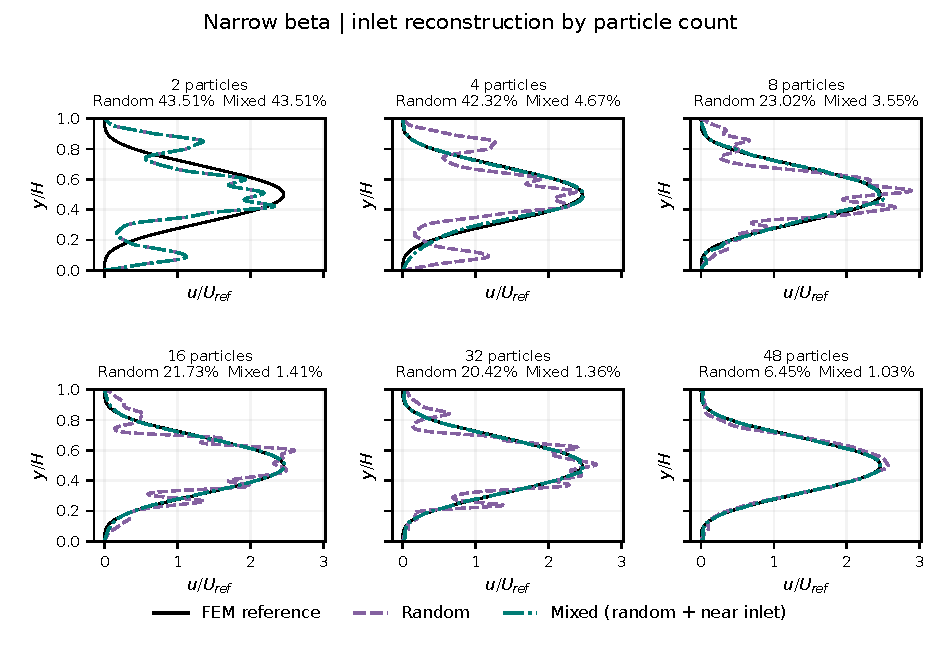
\includegraphics[width=\textwidth]{New_Adaptive_Particle_Results/inverse_rewrite/figures/beta5.pdf}
\caption{مقایسهٔ رهاسازی تصادفی و ترکیبی برای ورودی بتای باریک.}
\label{fig:inverse-rewrite-beta5}
\end{figure}
\FloatBarrier
شکل~\ref{fig:inverse-rewrite-skew_b3} بازسازی ورودی نامتقارن را مقایسه می‌کند.
در $48$ ذره، خطاهای تصادفی و ترکیبی $6.88\%$ و $1.04\%$ بودند.
\begin{figure}[htbp]
\centering
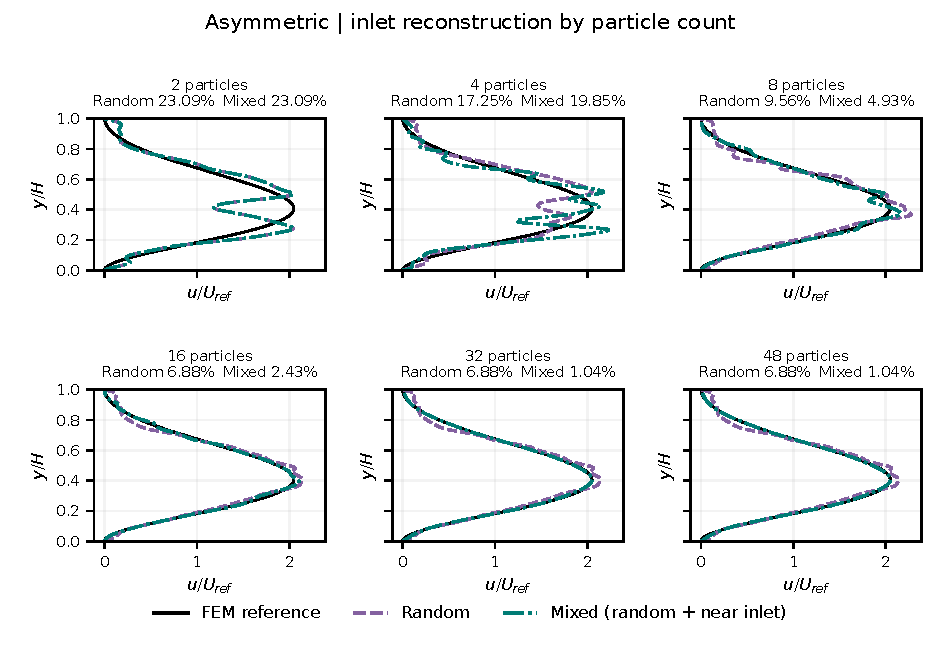
\includegraphics[width=\textwidth]{New_Adaptive_Particle_Results/inverse_rewrite/figures/skew_b3.pdf}
\caption{مقایسهٔ رهاسازی تصادفی و ترکیبی برای ورودی نامتقارن.}
\label{fig:inverse-rewrite-skew_b3}
\end{figure}
\FloatBarrier
شکل~\ref{fig:inverse-rewrite-flat30} بازسازی ورودی تقریباً تخت را مقایسه می‌کند.
در $48$ ذره، خطاهای تصادفی و ترکیبی $7.41\%$ و $3.84\%$ بودند.
\begin{figure}[htbp]
\centering
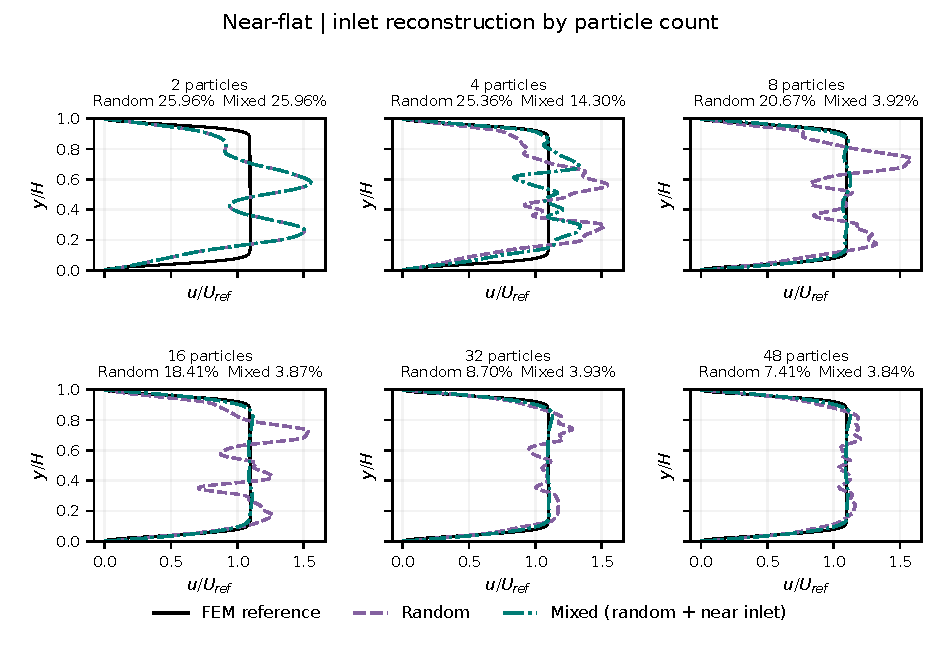
\includegraphics[width=\textwidth]{New_Adaptive_Particle_Results/inverse_rewrite/figures/flat30.pdf}
\caption{مقایسهٔ رهاسازی تصادفی و ترکیبی برای ورودی تقریباً تخت.}
\label{fig:inverse-rewrite-flat30}
\end{figure}
\FloatBarrier
شکل~\ref{fig:inverse-rewrite-twin_b3_r30} بازسازی ورودی دوقله‌ای را مقایسه می‌کند.
در $48$ ذره، خطاهای تصادفی و ترکیبی $9.34\%$ و $0.66\%$ بودند.
\begin{figure}[htbp]
\centering
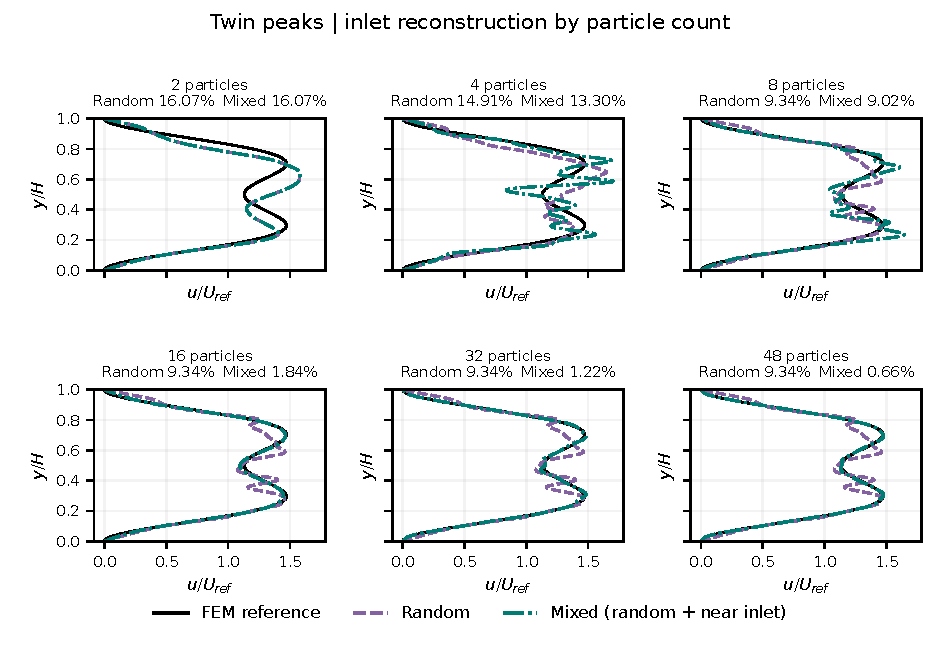
\includegraphics[width=\textwidth]{New_Adaptive_Particle_Results/inverse_rewrite/figures/twin_b3_r30.pdf}
\caption{مقایسهٔ رهاسازی تصادفی و ترکیبی برای ورودی دوقله‌ای.}
\label{fig:inverse-rewrite-twin_b3_r30}
\end{figure}
\FloatBarrier
شکل~\ref{fig:inverse-rewrite-shoulder} بازسازی ورودی شانه‌دار را مقایسه می‌کند.
در $48$ ذره، خطاهای تصادفی و ترکیبی $26.27\%$ و $1.90\%$ بودند.
\begin{figure}[htbp]
\centering
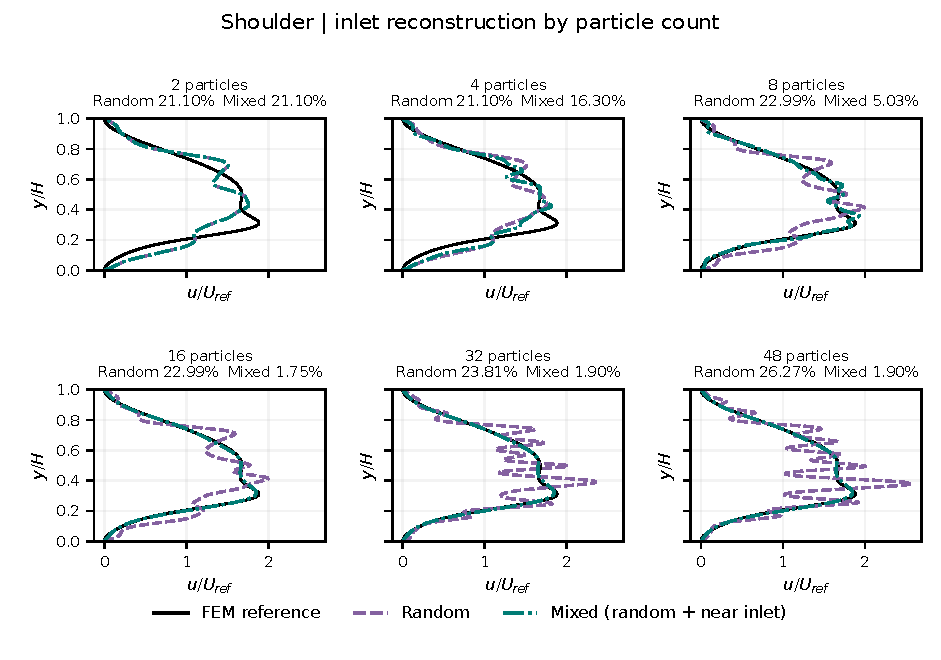
\includegraphics[width=\textwidth]{New_Adaptive_Particle_Results/inverse_rewrite/figures/shoulder.pdf}
\caption{مقایسهٔ رهاسازی تصادفی و ترکیبی برای ورودی شانه‌دار.}
\label{fig:inverse-rewrite-shoulder}
\end{figure}
\FloatBarrier
شکل~\ref{fig:inverse-rewrite-mixed} بازسازی ورودی چندمقیاسی را مقایسه می‌کند.
در $48$ ذره، خطاهای تصادفی و ترکیبی $14.55\%$ و $1.63\%$ بودند.
\begin{figure}[htbp]
\centering
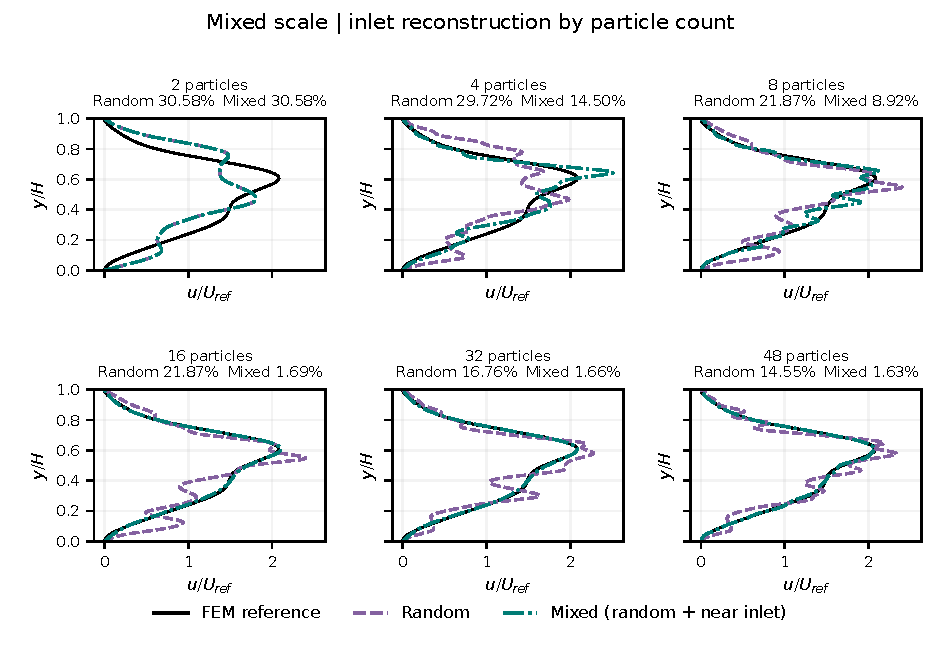
\includegraphics[width=\textwidth]{New_Adaptive_Particle_Results/inverse_rewrite/figures/mixed.pdf}
\caption{مقایسهٔ رهاسازی تصادفی و ترکیبی برای ورودی چندمقیاسی.}
\label{fig:inverse-rewrite-mixed}
\end{figure}
\FloatBarrier
شکل~\ref{fig:inverse-rewrite-waves3_r30} بازسازی ورودی سه‌نوسانی را مقایسه می‌کند.
در $48$ ذره، خطاهای تصادفی و ترکیبی $7.53\%$ و $1.48\%$ بودند.
\begin{figure}[htbp]
\centering
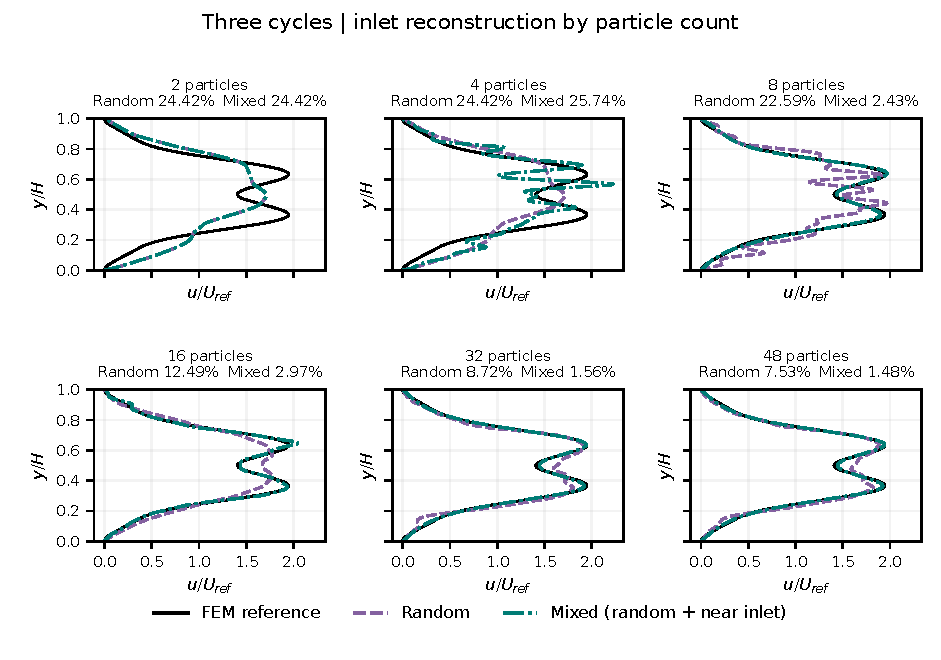
\includegraphics[width=\textwidth]{New_Adaptive_Particle_Results/inverse_rewrite/figures/waves3_r30.pdf}
\caption{مقایسهٔ رهاسازی تصادفی و ترکیبی برای ورودی سه‌نوسانی.}
\label{fig:inverse-rewrite-waves3_r30}
\end{figure}
\FloatBarrier
شکل~\ref{fig:inverse-rewrite-lobes4_r30} بازسازی ورودی چهارنوسانی را مقایسه می‌کند.
در $48$ ذره، خطاهای تصادفی و ترکیبی $16.42\%$ و $2.35\%$ بودند.
\begin{figure}[htbp]
\centering
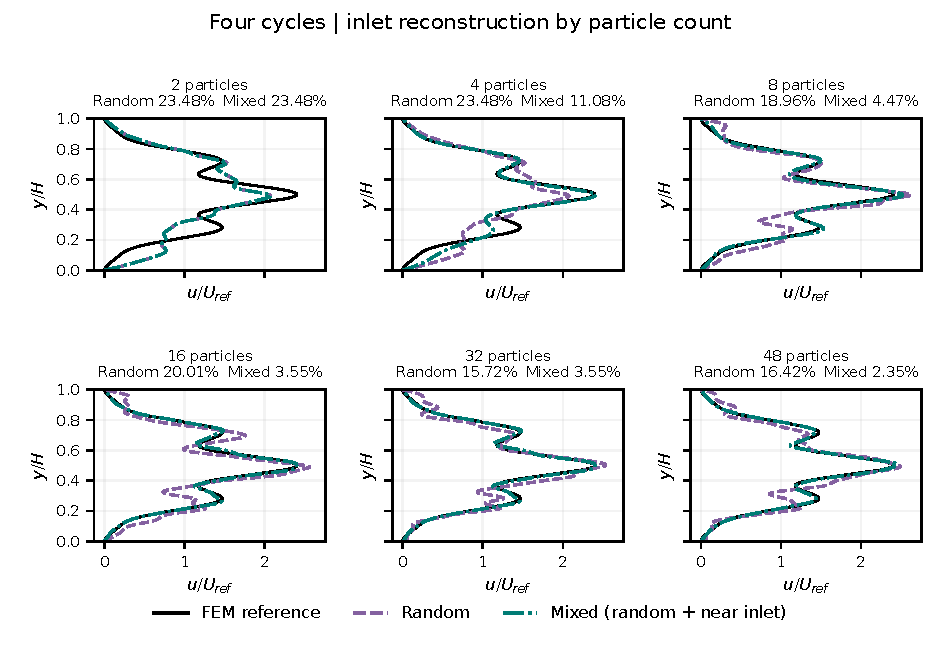
\includegraphics[width=\textwidth]{New_Adaptive_Particle_Results/inverse_rewrite/figures/lobes4_r30.pdf}
\caption{مقایسهٔ رهاسازی تصادفی و ترکیبی برای ورودی چهارنوسانی.}
\label{fig:inverse-rewrite-lobes4_r30}
\end{figure}
\FloatBarrier
شکل~\ref{fig:inverse-rewrite-nine30} بازسازی ورودی نه‌نوسانی را مقایسه می‌کند.
در $48$ ذره، خطاهای تصادفی و ترکیبی $38.93\%$ و $11.64\%$ بودند.
\begin{figure}[htbp]
\centering
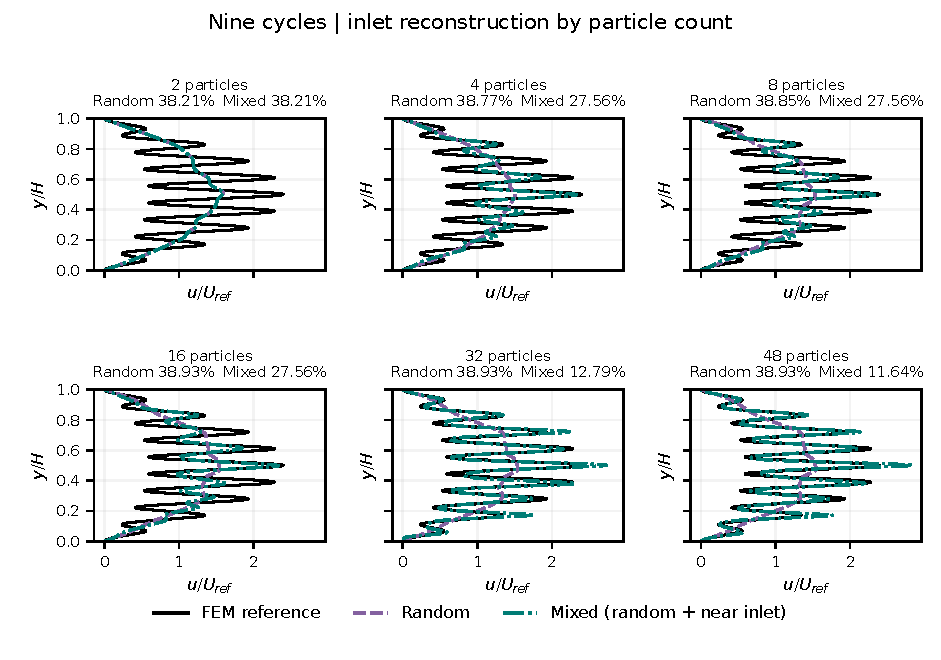
\includegraphics[width=\textwidth]{New_Adaptive_Particle_Results/inverse_rewrite/figures/nine30.pdf}
\caption{مقایسهٔ رهاسازی تصادفی و ترکیبی برای ورودی نه‌نوسانی.}
\label{fig:inverse-rewrite-nine30}
\end{figure}
\FloatBarrier
\par\medskip
\noindent\textbf{برآورد مستقیم ورودی از حرکت آغازین.}\par\smallskip
برای ورودی نه‌نوسانی، تنها بخش آغازین مسیرهای نزدیک ورودی بررسی شد.
معادلهٔ انتگرالی ذره برای برازش اسپلاین نامنفی به کار رفت.
تغییر سرعت در امتداد کانال با یک جملهٔ درجه‌دو تقریب زده شد.
انتخاب مدل با مسیرهای اعتبارسنجی و در پنجرهٔ مکانی مشترک انجام شد.
برای بررسی وضوح، اسپلاین‌های $45$ و $53$ ضریبی نیز آزموده شدند.
شکل~\ref{fig:inverse-rewrite-local} برآورد مستقیم ورودی را در دو تکرار نشان می‌دهد.
در $31$ ذره، خطاهای دو تکرار $4.08\%$ و $7.66\%$ بودند.
در $96$ ذره، خطاهای دو تکرار $3.18\%$ و $4.73\%$ بودند.
بازپخش کامل کانال با اپراتور ثابت جداگانه ارزیابی شد.
\begin{figure}[htbp]
\centering
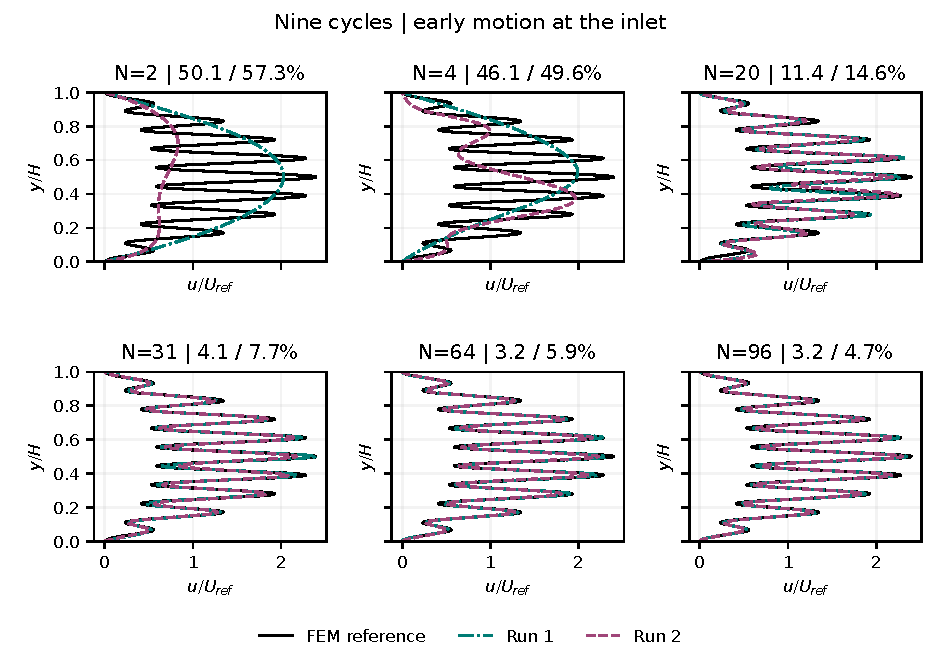
\includegraphics[width=\textwidth]{New_Adaptive_Particle_Results/inverse_rewrite/figures/nine30_local_inlet.pdf}
\caption{بازسازی موضعی ورودی نه‌نوسانی با مسیرهای نزدیک ورودی.}
\label{fig:inverse-rewrite-local}
\end{figure}
\FloatBarrier
